\documentclass{beamer}
\usepackage{graphicx}
\usepackage{hyperref}
\usepackage{diagbox}
\usepackage{colortbl}
\beamertemplatenavigationsymbolsempty
\setbeamertemplate{bibliography item}[triangle]
\setbeamertemplate{footline}
{
        \insertshorttitle 
        \hfill
        \insertframenumber{} / \inserttotalframenumber\hspace*{2ex} 
}



\title{Online Outlier Exploration over Large Datasets}
\author[Hansen]{Matthias Hansen \texttt{(matthias.hansen@rwth-aachen.de)} \\
        Advisor: Dr. Ines F\"arber}
\date{Seminar on Data Mining and Multimedia Search\\
        10.02.2015}
\institute{RWTH Aachen University}
\begin{document}

\frame{\titlepage}

\begin{frame}{Motivation}
    \centering{Why do Outlier Detection?}
\end{frame}
\section{Outlier Detection}
\begin{frame}{Example: Gaussian Distribution $\mathcal{N}(0,1)$}
    \centering
    \includegraphics<1>[width=.7\textwidth]{images/gaussian.png}
    \includegraphics<2>[width=.7\textwidth]{images/gaussian_lines.png}


    \visible<2>{Draw red lines at some arbitrary value for P(x).
        
    Within lines $\implies$ inlier.

    Outside lines $\implies$ outlier.}
\end{frame}
%\begin{frame}{The Traditional Approach: Statistical Distributions}
%    \begin{itemize}
%        \item Statistical Distribution of Data must be known.
%        \item Linear Runtime.
%        \item Distribution can sometimes be Inferred (e.g. using Expectation Maximization).
%    \end{itemize}
%\end{frame}
\begin{frame}{Counterexample: Geospatial Data}
    \begin{itemize}
        \item OpenStreetMap Data for South America and South Pacific
        \item Roughly 1.3 Gigabytes of Data (Raw Positions)

    \end{itemize}
    \begin{center}
    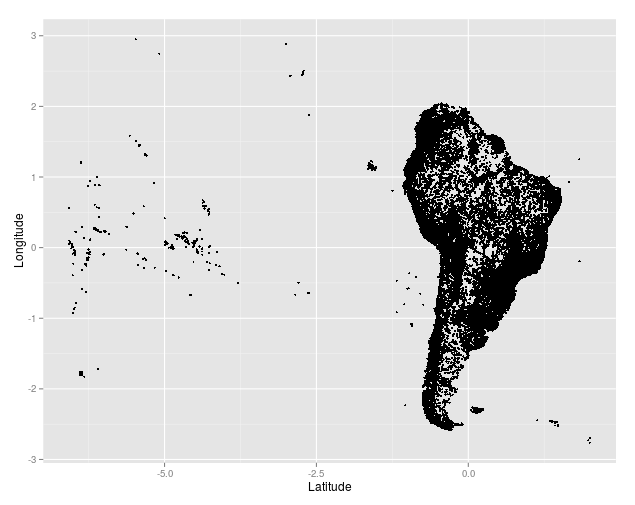
\includegraphics[width=.7\textwidth]{images/south_america.png} 
    \end{center}
\end{frame}
\begin{frame}{Counterexample: Geospatial Data}
    \begin{center}
    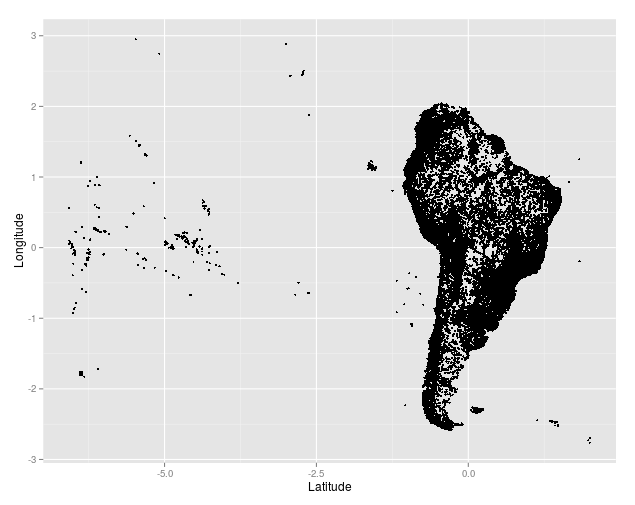
\includegraphics[width=.7\textwidth]{images/south_america.png} 
    \end{center}
    \begin{itemize}
        \item Task: Find wrong data inserted by malicious users.

        \item Example: Someone placed a shop in the middle of the ocean.

    \end{itemize}
\end{frame}
\begin{frame}{Distance-Based Outliers}
    \begin{block}{Distance-Based Outliers}
        $p\in DB$ is distance-based outlier w.r.t. $k$ and $\varepsilon$
        iff. $|\{q\in DB | dist(p,q) < \varepsilon\}| < k$
    \end{block}

    \begin{itemize}
        \item Same notion as ``non-core points'' in DBSCAN.
        \item Meaningful for geospatial data with Euclidean Distance.
    \end{itemize}
    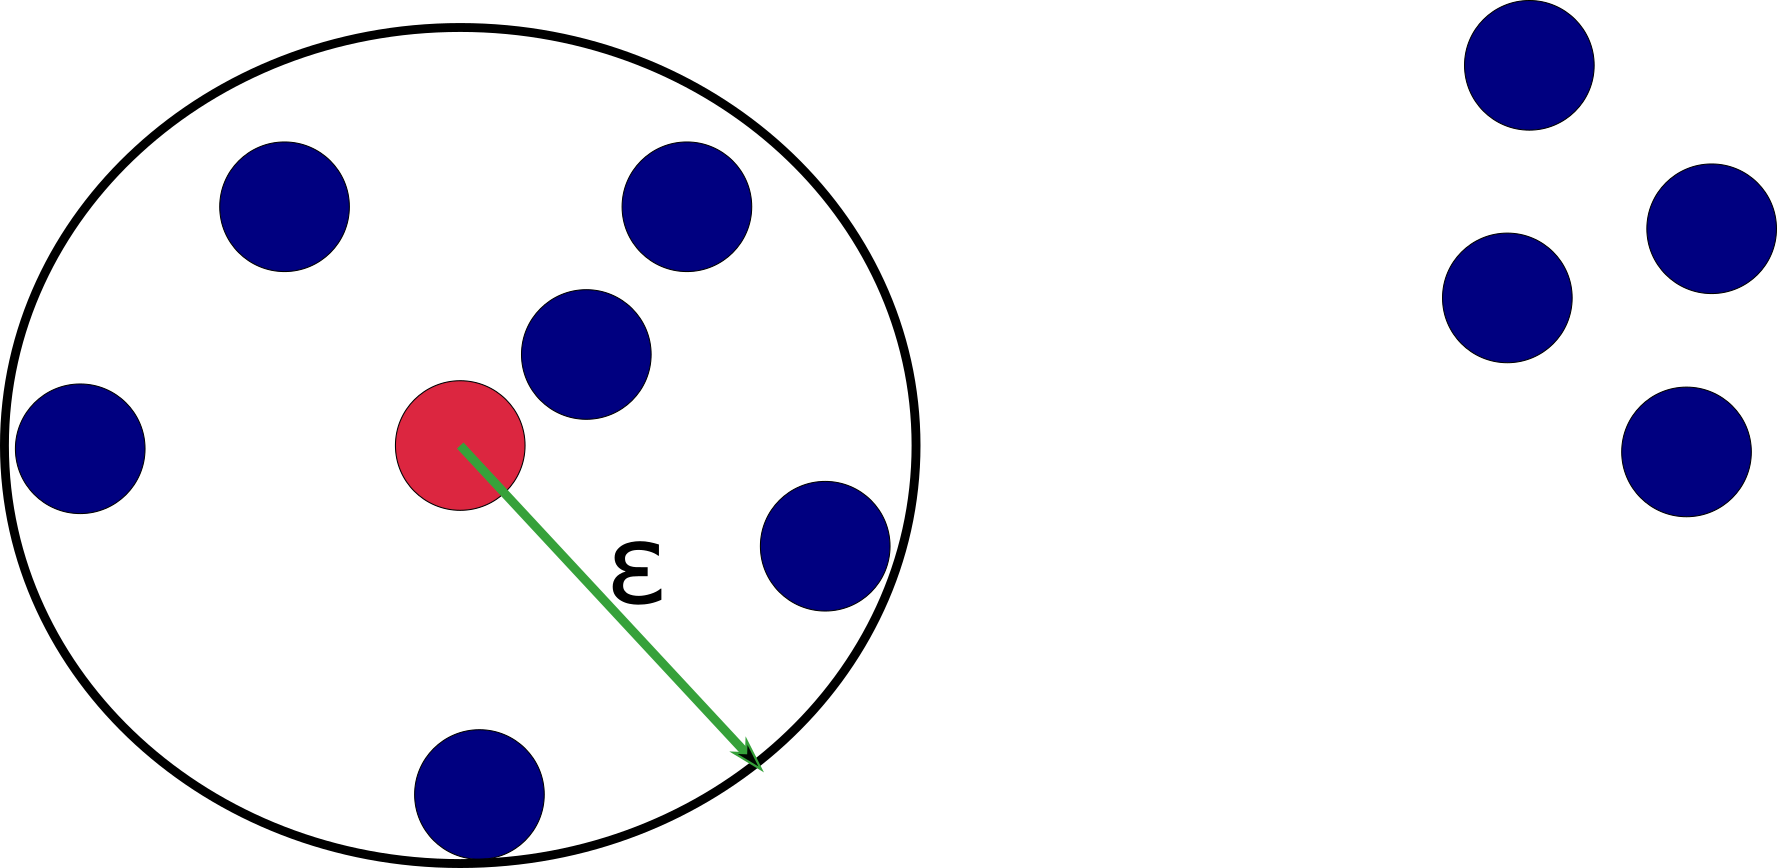
\includegraphics[width=.5\textwidth]{images/dboutliers.png}
    \begin{itemize}
        \item Alternative definition: $k$-th neighbor is closer than $\varepsilon$
    \end{itemize}
    
\end{frame}
\section{Outlier Detection and Performance}
\begin{frame}{Performance Considerations}
    \begin{itemize}
        \item Naive: Calculate all pairwise distances. ($\mathcal{O}(n^2)$)

               Check criterion for each point.
        \item Better: Insert data into spatial index structure. 

              Compute $k$-nearest neighbors. 

              Check whether distance to $k$-th neighbor is $\leq$ $\varepsilon$.

          \item Runtime in $\mathcal{O}(n\log(n))$ 
              
              (except for some high-dimensional cases)
    \end{itemize}
\end{frame}
\begin{frame}{A First Attempt\ldots}
    Select some parameters: \visible<2>{\alert{Maybe $k = 5$ and $\varepsilon = 0.0001$?}}
    \begin{center}
        \visible{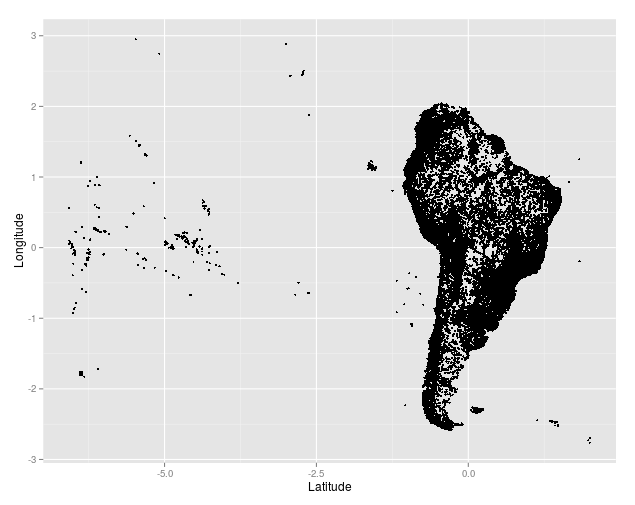
\includegraphics[width=.8\textwidth]{images/south_america.png}}
    \end{center}
\end{frame}
\begin{frame}{A First Attempt\ldots}
    Select some parameters: \alert{Maybe $k = 5$ and $\varepsilon = 0.0001$}?
    \begin{center}\visible<1>{
    Wait for a while\ldots}\end{center}
    \begin{center}
        \visible<2>{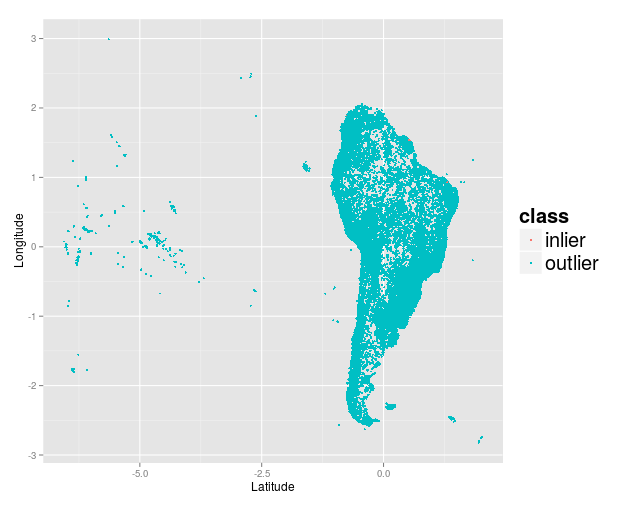
\includegraphics[width=.8\textwidth]{images/south_america_outliers.png}}
    \end{center}
\end{frame}
\begin{frame}{Parameter Selection is a Problem}
    \begin{itemize}
        \item Good parameter setting not obvious. 
        \item Settings can not be tested on Subsets: \alert{Results will differ!}
        \item Solution?\pause

        \item ONION (\underline{On}line Outlier Detect\underline{ion}) system:

            Store intermediate results. 

            $\rightarrow$ Detect Outliers in logarithmic time.
    \end{itemize}
\end{frame}
\begin{frame}{A Small Example}
    Consider the following dataset:
    \begin{columns}
        \begin{column}{.7\textwidth}
            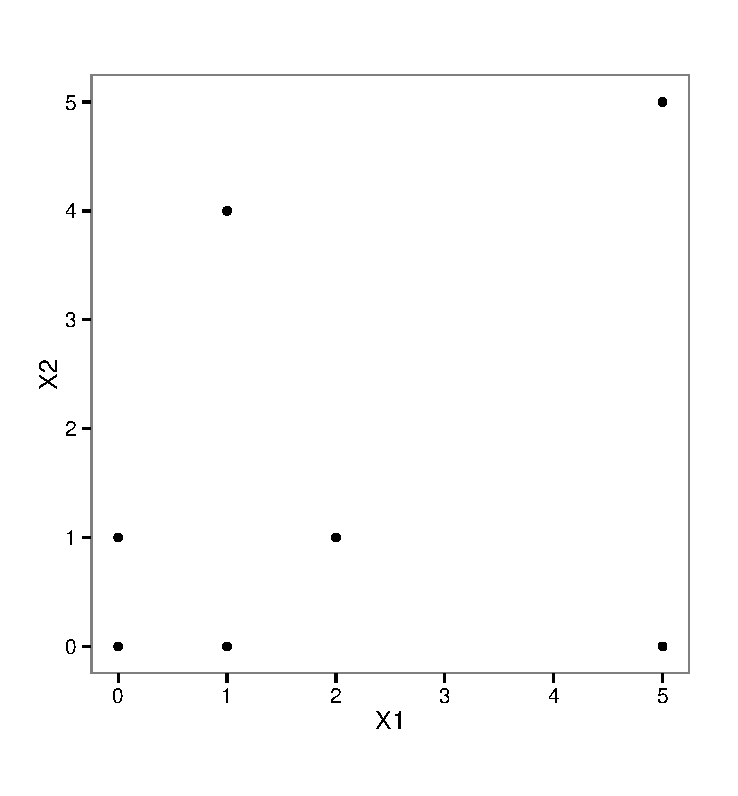
\includegraphics[width=.7\linewidth]{images/example_plot.eps}
        \end{column}
        \begin{column}{.3\textwidth}
            \begin{tabular}{ | c | c  c |}
            \hline
            i & X1 & X2 \\
            \hline
            0 & 0 & 0 \\
            1 & 1 & 0 \\
            2 & 0 & 1 \\
            3 & 5 & 0 \\
            4 & 1 & 4 \\
            5 & 2 & 1 \\
            6 & 5 & 5 \\
            \hline
            \end{tabular}
        \end{column}
    \end{columns}
    Say we want to perform outlier detection with $k=4$ and $\varepsilon=3.5$
\end{frame}
\begin{frame}{A Small Example (continued)}
    Say we want to perform outlier detection with $k=4$ and $\varepsilon=3.5$
    $K$-Nearest-Neighbors query yields:
    \begin{tabular}{|c|c|c|c|c|}
        \hline
        \backslashbox{i}{k} & 1 & 2 & 3 & 4 \\
        \hline
        0 &  0 &  1.000000 &  1.000000 &  2.236068 \\
        1 &  0 &  1.000000 &  1.414214 &  1.414214 \\
        2 &  0 &  1.000000 &  1.414214 &  2.000000\\
        3 &  0 &  3.162278 &  4.000000 &  5.000000 \\
        4 &  0 &  3.162278 &  3.162278 &  4.000000 \\
        5 &  0 &  1.414214 &  2.000000 &  2.236068 \\
        6 &  0 &  4.123106 &  5.000000 &  5.000000 \\
        \hline
     \end{tabular}
\end{frame}
\begin{frame}{A Small Example (continued)}
    Say we want to perform outlier detection with $k=4$ and $\varepsilon=3.5$
    $K$-Nearest-Neighbors query yields:
    \begin{tabular}{|c|c|c|c|>{\columncolor[rgb]{1,0.5,0.5}}c|}
        \hline
        \backslashbox{i}{k} & 1 & 2 & 3 & 4 \\
        \hline
        0 &  0 &  1.000000 &  1.000000 &  2.236068 \\
        1 &  0 &  1.000000 &  1.414214 &  1.414214 \\
        2 &  0 &  1.000000 &  1.414214 &  2.000000\\
        3 &  0 &  3.162278 &  4.000000 &  5.000000 \\
        4 &  0 &  3.162278 &  3.162278 &  4.000000 \\
        5 &  0 &  1.414214 &  2.000000 &  2.236068 \\
        6 &  0 &  4.123106 &  5.000000 &  5.000000 \\
        \hline
     \end{tabular}
     \pause

     We can now re-use this table, right?\pause

     \alert{Table size too big!}
\end{frame}
\begin{frame}{New Approach: Ranges for $\varepsilon$ and $k$}
    Let $k = [k_{min},k_{max}] = [3,4]$

    and $\varepsilon = [\varepsilon_{min},\varepsilon_{max}] = [2,3.5]$

    Now prune the table:

    \only<1>{\begin{tabular}{|c|c|c|c|c|}
        \hline
        \backslashbox{i}{k} & 1 & 2 & 3 & 4 \\
        \hline
        0 &  0 &  1.000000 &  1.000000 &  2.236068 \\
        1 &  0 &  1.000000 &  1.414214 &  1.414214 \\
        2 &  0 &  1.000000 &  1.414214 &  2.000000 \\
        3 &  0 &  3.162278 &  4.000000 &  5.000000 \\
        4 &  0 &  3.162278 &  3.162278 &  4.000000 \\
        5 &  0 &  1.414214 &  2.000000 &  2.236068 \\
        6 &  0 &  4.123106 &  5.000000 &  5.000000 \\
        \hline
    \end{tabular}}

    \only<2>{\begin{tabular}{|c|c|c|}
        \hline
        \backslashbox{i}{k} & 3 & 4 \\
        \hline
        0 & 1.000000 &  2.236068 \\
        1 & 1.414214 &  1.414214 \\
        2 & 1.414214 &  2.000000 \\
        3 & 4.000000 &  5.000000 \\
        4 & 3.162278 &  4.000000 \\
        5 & 2.000000 &  2.236068 \\
        6 & 5.000000 &  5.000000 \\
        \hline
    \end{tabular}}

    \only<3>{\begin{tabular}{|c|c|c|}
        \hline
        \backslashbox{i}{k} & 3 & 4 \\
        \hline
        0 & 1.000000 &  2.236068 \\
        1 & \multicolumn{2}{|c|}{\textit{Const Inlier}} \\
        2 & \multicolumn{2}{|c|}{\textit{Const Inlier}} \\
        3 & \multicolumn{2}{|c|}{\textit{Const Outlier}} \\
        4 & 3.162278 &  4.000000 \\
        5 & 2.000000 &  2.236068 \\
        6 & \multicolumn{2}{|c|}{\textit{Const Outlier}} \\
        \hline
    \end{tabular}}
    \only<4>{
        \begin{columns}
            \begin{column}{.5\textwidth}
                \begin{tabular}{|c|c|c|}
                    \hline
                    \backslashbox{i}{k} & 3 & 4 \\
                    \hline
                    0 & 1.000000 &  2.236068 \\
                    1 & \multicolumn{2}{|c|}{\textit{Const Inlier}} \\
                    2 & \multicolumn{2}{|c|}{\textit{Const Inlier}} \\
                    3 & \multicolumn{2}{|c|}{\textit{Const Outlier}} \\
                    4 & 3.162278 &  4.000000 \\
                    5 & 2.000000 &  2.236068 \\
                    6 & \multicolumn{2}{|c|}{\textit{Const Outlier}} \\
                    \hline
                \end{tabular}
            \end{column}
            \begin{column}{.5\textwidth}
                \begin{tabular}{|c|c|}
                    \hline
                    id & class \\
                    \hline
                    0 & \textit{Outlier Candidate} \\
                    1 & \textit{Const Inlier} \\
                    2 & \textit{Const Inlier} \\
                    3 & \textit{Const Outlier} \\
                    4 & \textit{Outlier Candidate} \\
                    5 & \textit{Outlier Candidate} \\
                    6 & \textit{Const Outlier} \\
                    \hline
                \end{tabular}
            \end{column}
        \end{columns}
    }
    
    \only<5>{
        \begin{columns}
            \begin{column}{.5\textwidth}
                \begin{tabular}{|c|c|c|}
                    \hline
                    \backslashbox{i}{k} & 3 & 4 \\
                    \hline
                    0 & 1.000000 &  2.236068 \\
                    4 & 3.162278 &  4.000000 \\
                    5 & 2.000000 &  2.236068 \\
                    \hline
                \end{tabular}
            \end{column}
            \begin{column}{.5\textwidth}
                \begin{tabular}{|c|c|}
                    \hline
                    id & class \\
                    \hline
                    0 & \textit{Outlier Candidate} \\
                    1 & \textit{Const Inlier} \\
                    2 & \textit{Const Inlier} \\
                    3 & \textit{Const Outlier} \\
                    4 & \textit{Outlier Candidate} \\
                    5 & \textit{Outlier Candidate} \\
                    6 & \textit{Const Outlier} \\
                    \hline
                \end{tabular}
            \end{column}
        \end{columns}
    }
    \only<5>{We refer to this data structure as \textit{O-Space} (ONION Space).}
\end{frame}
\begin{frame}
    Outlier Detection using \textit{O-Space} is still linear.

    Can we do even better?\pause

    Maybe with Sorting?
\end{frame}
\begin{frame}
    \only<1>{
        \begin{columns}
            \begin{column}{.5\textwidth}
                \begin{tabular}{|c|c|c|}
                    \hline
                    \backslashbox{i}{k} & 3 & 4 \\
                    \hline
                    0 & 1.000000 &  2.236068 \\
                    4 & 3.162278 &  4.000000 \\
                    5 & 2.000000 &  2.236068 \\
                    \hline
                \end{tabular}
            \end{column}
            \begin{column}{.5\textwidth}
                \begin{tabular}{|c|c|}
                    \hline
                    id & class \\
                    \hline
                    0 & \textit{Outlier Candidate} \\
                    1 & \textit{Const Inlier} \\
                    2 & \textit{Const Inlier} \\
                    3 & \textit{Const Outlier} \\
                    4 & \textit{Outlier Candidate} \\
                    5 & \textit{Outlier Candidate} \\
                    6 & \textit{Const Outlier} \\
                    \hline
                \end{tabular}
            \end{column}
        \end{columns}
    }
    \only<2>{
        \begin{columns}
            \begin{column}{.5\textwidth}
                \begin{tabular}{|c|c|}
                    \hline
                    3 & 4 \\
                    \hline
                    (0,1.000000) &  (0,2.236068) \\
                    (4,3.162278) &  (4,4.000000) \\
                    (5,2.000000) &  (5,2.236068) \\
                    \hline
                \end{tabular}
            \end{column}
            \begin{column}{.5\textwidth}
                \begin{tabular}{|c|c|}
                    \hline
                    id & class \\
                    \hline
                    0 & \textit{Outlier Candidate} \\
                    1 & \textit{Const Inlier} \\
                    2 & \textit{Const Inlier} \\
                    3 & \textit{Const Outlier} \\
                    4 & \textit{Outlier Candidate} \\
                    5 & \textit{Outlier Candidate} \\
                    6 & \textit{Const Outlier} \\
                    \hline
                \end{tabular}
            \end{column}
        \end{columns}
    }
    \only<3>{
        \begin{columns}
            \begin{column}{.5\textwidth}
                \begin{tabular}{|c|c|}
                    \hline
                    3 & 4 \\
                    \hline
                    (0,1.000000) &  (5,2.236068) \\
                    (5,2.000000) &  (0,2.236068) \\
                    (4,3.162278) &  (4,4.000000) \\
                    \hline
                \end{tabular}
            \end{column}
            \begin{column}{.5\textwidth}
                \begin{tabular}{|c|c|}
                    \hline
                    id & class \\
                    \hline
                    0 & \textit{Outlier Candidate} \\
                    1 & \textit{Const Inlier} \\
                    2 & \textit{Const Inlier} \\
                    3 & \textit{Const Outlier} \\
                    4 & \textit{Outlier Candidate} \\
                    5 & \textit{Outlier Candidate} \\
                    6 & \textit{Const Outlier} \\
                    \hline
                \end{tabular}
            \end{column}
        \end{columns}

        \vspace{1cm}
        This data structure is called \textbf{P-Space}.
    }
    \end{frame}
    \begin{frame}{Contributions}
        \begin{itemize}
            \item Logarithmic-time outlier detection 
                \begin{itemize}
                   \item $\mathcal{O}(\log(|OC|))$
                    \item By storing a large data structure in memory.
                    \item After some initial setup time.
                    \item For a limited parameter range.
                \end{itemize}
            \item What else?
        \end{itemize}
    \end{frame}
    \begin{frame}{Other Useful Operations}
    \begin{center}
        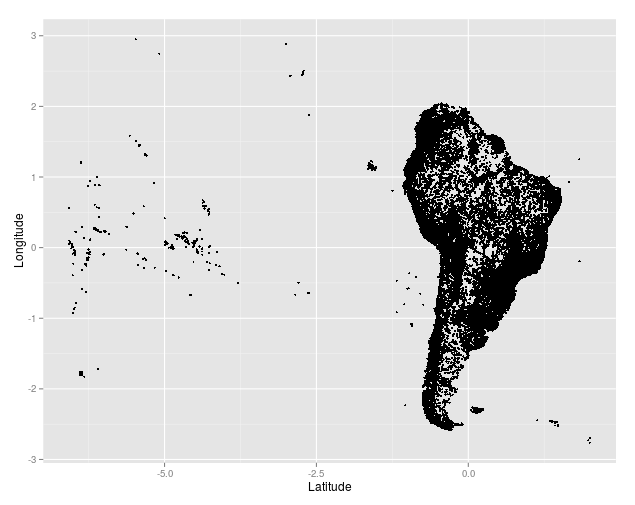
\includegraphics[width=\textwidth]{images/south_america.png}
    \end{center}
    Guessing is one way to find a parameter setting. Should there be others?
    \end{frame}
\section{Comparative Outliers}
    \begin{frame}{Comparative Outliers}
        Given a set of outliers, which other points must also be outliers?

        Formally: Let P $\subseteq DB$. 
        
        Find \alert<2>{maximal} Q, such that 
        
        $\forall (k,\varepsilon) (\text{All } p \in P \text{ are outliers } \implies \text{All } q \in Q \text{ are outliers})$
    \end{frame}
%    \begin{frame}
%    \only<1>{
%        \begin{columns}
%            \begin{column}{.5\textwidth}
%                \begin{tabular}{|c|c|}
%                    \hline
%                    3 & 4 \\
%                    \hline
%                    (0,1.000000) &  (5,2.236068) \\
%                    (5,2.000000) &  (0,2.236068) \\
%                    (4,3.162278) &  (4,4.000000) \\
%                    \hline
%                \end{tabular}
%            \end{column}
%            \begin{column}{.5\textwidth}
%                \begin{tabular}{|c|c|}
%                    \hline
%                    id & class \\
%                    \hline
%                    0 & \textit{Outlier Candidate} \\
%                    1 & \textit{Const Inlier} \\
%                    2 & \textit{Const Inlier} \\
%                    3 & \textit{Const Outlier} \\
%                    4 & \textit{Outlier Candidate} \\
%                    5 & \textit{Outlier Candidate} \\
%                    6 & \textit{Const Outlier} \\
%                    \hline
%                \end{tabular}
%            \end{column}
%        \end{columns}
%    }
%    \only<2>{
%        \begin{columns}
%            \begin{column}{.5\textwidth}
%                \begin{tabular}{|c|c|}
%                    \hline
%                    3 & 4 \\
%                    \hline
%                    \cellcolor{blue} (0,1.000000) & \cellcolor{red} (5,2.236068) \\
%                    (5,2.000000)\cellcolor{red} &  \cellcolor{blue}(0,2.236068) \\
%                    \cellcolor{green} (4,3.162278) &  \cellcolor{green}(4,4.000000) \\
%                    \hline
%                \end{tabular}
%            \end{column}
%            \begin{column}{.5\textwidth}
%                \begin{tabular}{|c|c|}
%                    \hline
%                    id & class \\
%                    \hline
%                    0 & \textit{Outlier Candidate} \\
%                    1 & \textit{Const Inlier} \\
%                    2 & \textit{Const Inlier} \\
%                    3 & \textit{Const Outlier} \\
%                    4 & \textit{Outlier Candidate} \\
%                    5 & \textit{Outlier Candidate} \\
%                    6 & \textit{Const Outlier} \\
%                    \hline
%                \end{tabular}
%            \end{column}
%        \end{columns}
%    }
%    \end{frame}
\begin{frame}{Example}
    \begin{columns}
        \begin{column}{.6\textwidth}
            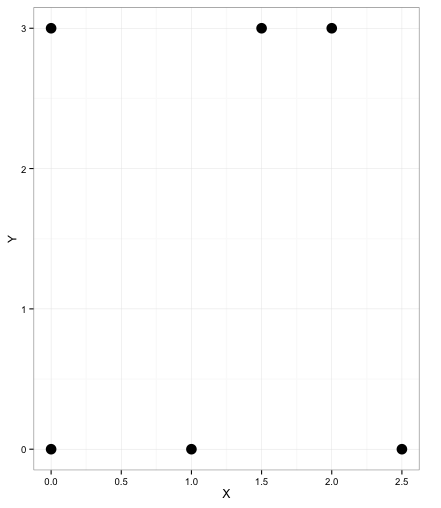
\includegraphics[height=.8\textheight]{images/counterexample.png}
        \end{column}
        \begin{column}{.4\textwidth}
            \begin{tabular}{| c | c |} 
                \hline
                \multicolumn{2}{| c |}{k}\\ 
                \hline
                2 & 3\\
                \hline
                (5,0.5) & (2,1.5)\\ 
                (6,0.5) & (5,1.5)\\ 
                (1,1) & (4,2)\\ 
                (2,1) & (6,2)\\ 
                (3,1.5) & (1,2.5)\\ 
                (4,1.5) & (3,2.5)\\ 
                \hline
            \end{tabular}

            \vspace{.5cm}

            \textbf{K-Domination:}
            
            $p \leq_k q \iff $

            $\forall\varepsilon (q\text{ is Outlier}\implies p\text{ is Outlier})$

            \textbf{(Full) Domination:}

            $p \leq q \iff $
            
            $\forall k (p \leq_k q)$
        \end{column}
    \end{columns}
\end{frame}
\begin{frame}{Example}
    \definecolor{einscol}{RGB}{241,97,96}
    \definecolor{zweicol}{RGB}{168,144,31}
    \definecolor{dreicol}{RGB}{38,176,54}
    \definecolor{viercol}{RGB}{40,179,183}
    \definecolor{funfcol}{RGB}{85,139,252}
    \definecolor{sechscol}{RGB}{237,78,220}
    \begin{columns}
        \begin{column}{.6\textwidth}
            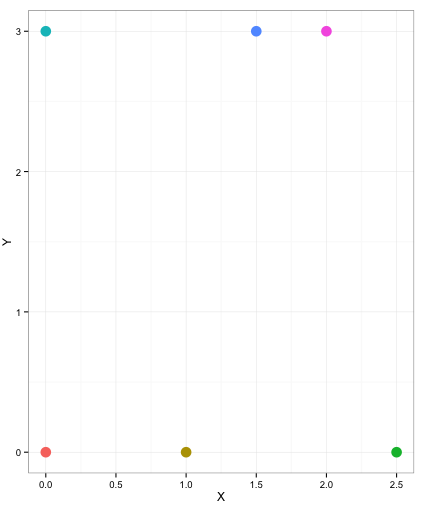
\includegraphics[height=.8\textheight]{images/counterexample_color.png}
        \end{column}
        \begin{column}{.4\textwidth}
            \begin{tabular}{| c | c |} 
                \hline
                \multicolumn{2}{| c |}{k}\\ 
                \hline
                2 & 3\\
                \hline
                \cellcolor{funfcol}(5,0.5) & \cellcolor{zweicol}(2,1.5)\\ 
                \cellcolor{sechscol}(6,0.5) & \cellcolor{funfcol}(5,1.5)\\ 
                \cellcolor{einscol}(1,1) & \cellcolor{viercol}(4,2)\\ 
                \cellcolor{zweicol}(2,1) & \cellcolor{sechscol}(6,2)\\ 
              \cellcolor{dreicol}  (3,1.5) &\cellcolor{einscol} (1,2.5)\\ 
                \cellcolor{viercol}(4,1.5) &\cellcolor{dreicol} (3,2.5)\\ 
                \hline
            \end{tabular}
            \vspace{.5cm}

            \textbf{K-Domination:}
            
            $p \leq_k q \iff $

            $\forall\varepsilon (q\text{ is Outlier}\implies p\text{ is Outlier})$

            \textbf{(Full) Domination:}

            $p \leq q \iff $
            
            $\forall k (p \leq_k q)$
        \end{column}
    \end{columns}
\end{frame}
\begin{frame}
    \definecolor{einscol}{RGB}{241,97,96}
    \definecolor{zweicol}{RGB}{168,144,31}
    \definecolor{dreicol}{RGB}{38,176,54}
    \definecolor{viercol}{RGB}{40,179,183}
    \definecolor{funfcol}{RGB}{85,139,252}
    \definecolor{sechscol}{RGB}{237,78,220}
    \begin{columns}
        \begin{column}{.5\textwidth}
            \begin{tabular}{| c | c |} 
                \hline
                \multicolumn{2}{| c |}{k}\\ 
                \hline
                2 & 3\\
                \hline
                \cellcolor{funfcol}(5,0.5) & \cellcolor{zweicol}(2,1.5)\\ 
                \cellcolor{sechscol}(6,0.5) & \cellcolor{funfcol}(5,1.5)\\ 
                \cellcolor{einscol}(1,1) & \cellcolor{viercol}(4,2)\\ 
                \cellcolor{zweicol}(2,1) & \cellcolor{sechscol}(6,2)\\ 
              \cellcolor{dreicol}  (3,1.5) &\cellcolor{einscol} (1,2.5)\\ 
                \cellcolor{viercol}(4,1.5) &\cellcolor{dreicol} (3,2.5)\\ 
                \hline
            \end{tabular}

           \ \\

            \textbf{K-Domination:}
            
            $p \leq_k q \iff $

            $\forall\varepsilon (q\text{ is Outlier}\implies p\text{ is Outlier})$

            \textbf{(Full) Domination:}

            $p \leq q \iff $
            
            $\forall k (p \leq_k q)$
        \end{column}
        \begin{column}{.5\textwidth}
            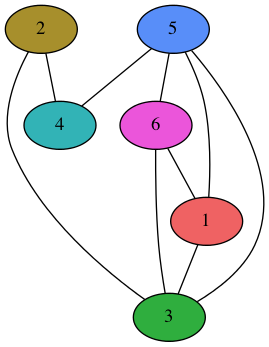
\includegraphics[width=\textwidth]{images/graph/graph.png}
        \end{column}
    \end{columns}
    \visible<2>{Decomposing means solving \textsc{Cliques} $\implies$ \alert{very slow}}
\end{frame}
    \begin{frame}{Contributions}
        \begin{itemize}
            \item Logarithmic-time Outlier Detection 
                \begin{itemize}
                   \item $\mathcal{O}(\log(|OC|))$
                    \item By storing a large data structure in memory.
                    \item After some initial setup time.
                    \item For a limited parameter range.
                \end{itemize}
            \item Comparative Outliers
                \begin{itemize}
                    \item $\mathcal{O}(|OC| \cdot k)$ using P-Space.
                    \item  $\mathcal{O}(\log(comp_1)+\log(comp_2)\ldots)$ D-Space and referring to O-Space.
                \end{itemize}
            \item What else?
        \end{itemize}
    \end{frame}
\begin{frame}
    ``Backwards Search'' for Outliers:
    
    Find $(k,\varepsilon)$, such that a all $p\in P$ are Outliers 

    (and the number of Outliers is minimal). \pause

    \begin{center}
    \begin{tabular}{| c | c |} 
        \hline
        \multicolumn{2}{| c |}{k}\\ 
        \hline
        2 & 3\\
        \hline
        (5,0.5) & (2,1.5)\\ 
        (6,0.5) & (5,1.5)\\ 
        (1,1) & (4,2)\\ 
        (2,1) & (6,2)\\ 
        (3,1.5) & (1,2.5)\\ 
        (4,1.5) & (3,2.5)\\ 
        \hline
    \end{tabular}
    \end{center}
    \pause
    \begin{itemize}
    \item The Paper calls this ``Outlier-Centric Parameter Space Exploration'' (PSE).
    \end{itemize}
\end{frame}
    \begin{frame}{Contributions}
        \begin{itemize}
            \item Logarithmic-time Outlier Detection 
               \begin{itemize}
                   \item $\mathcal{O}(\log(|OC|))$
                    \item By storing a large data structure in memory.
                    \item After some initial setup time.
                    \item For a limited parameter range.
                \end{itemize}
           \item Comparative Outliers
                \begin{itemize}
                    \item $\mathcal{O}(|OC| \cdot k)$ using P-Space.
                    \item  $\mathcal{O}(\log(comp_1)+\log(comp_2)\ldots)$ D-Space and referring to O-Space.
                \end{itemize}
            \item Parameter Space Exploration
                    \begin{itemize}
                    \item $\mathcal{O}(k\cdot |OC|)$ using P-Space.
                    \item $\mathcal{O}(k\cdot |P|)$ using O-Space.
                   \end{itemize}
        \end{itemize}
    \end{frame}
\begin{frame}{Criticism}
\begin{itemize}
\item New Operations very helpful.
\item Faster Outlier Detection. 
\end{itemize}
But:
\begin{itemize}
\item Only really applicable if data fits into memory of a single machine.
\item Preprocessing takes long.
\item Results of preprocessing useless unless parameters chosen carefully.
\item D-Space construction only useful when $k_{max} - k_{min}$ very big.
\end{itemize}
\end{frame}
\appendix
\begin{frame}{References}
\nocite{onion,dolphin,parallel_knn,kriegeldefinitions}
\def\newblock{}
\bibliographystyle{plain}
\bibliography{References}
\end{frame}    



\end{document}
